\documentclass[10pt]{beamer}

\usepackage{arxiv}

\usepackage[T2A]{fontenc}
\usepackage[utf8]{inputenc}
\usepackage[english, russian]{babel}
% \usepackage{cmap}
\usepackage{url}
\usepackage{booktabs}
\usepackage{nicefrac}
\usepackage{microtype}
\usepackage{lipsum}
\usepackage{graphicx}
\usepackage{subfig}
\usepackage[square,sort,comma,numbers]{natbib}
\usepackage{doi}
\usepackage{multicol}
\usepackage{multirow}
\usepackage{tabularx}

\usepackage{tikz}
\usetikzlibrary{matrix}

% Algorithms
\usepackage{algpseudocode}
\usepackage{algorithm}

%% Шрифты
\usepackage{euscript} % Шрифт Евклид
\usepackage{mathrsfs} % Красивый матшрифт
\usepackage{extsizes}

\usepackage{makecell} % diaghead in a table
\usepackage{amsmath,amsfonts,amssymb,amsthm,mathtools,dsfont}
\usepackage{icomma}

\usepackage{hyperref}
% \usepackage[usenames,dvipsnames,svgnames,table,rgb]{xcolor}

\hypersetup{
	unicode=true,
	pdftitle={Байесовский подход к выбору достаточного размера выборки},
	pdfauthor={Киселев Никита Сергеевич},
	pdfkeywords={определение размера выборки, байесовский подход},
	colorlinks=true,
	linkcolor=black,        % внутренние ссылки
	citecolor=green,         % на библиографию
	filecolor=magenta,      % на файлы
	urlcolor=blue           % на URL
}

\graphicspath{{./figures/}}

\usepackage{enumitem} % Для модификаций перечневых окружений
\usepackage{etoolbox}

\makeatletter
\expandafter\patchcmd\csname\string\algorithmic\endcsname{\itemsep\z@}{\itemsep=1.5mm}{}{}
\makeatother

% Теоремы
\newtheorem{theorem}{Теорема}
\newtheorem{lemma}{Лемма}
\newtheorem{proposition}{Утверждение}
\newtheorem*{exercise}{Упражнение}
\newtheorem*{problem}{Задача}

\newtheorem{definition}{Определение}
\newtheorem*{corollary}{Следствие}
\newtheorem*{note}{Замечание}
\newtheorem*{reminder}{Напоминание}
\newtheorem*{example}{Пример}
\newtheorem*{cexample}{Контрпример}
\newtheorem*{solution}{Решение}

\renewcommand{\abstractname}{Аннотация}

% математический шрифт как в article
\usefonttheme[onlymath]{serif}

\title[\hbox to 56mm{Байесовский подход к выбору достаточного размера выборки\hfill\insertframenumber\,/\,\inserttotalframenumber}]{\vspace{1cm} \\ \LARGE{\textbf{Байесовский подход к выбору достаточного размера выборки}}}

\author[Никита Киселев]{
Киселев Никита Сергеевич\\
\vspace{0.5cm}
\footnotesize{Научный руководитель:\\
к.ф.-м.н. А.\,В.\,Грабовой}
}
    
\institute[МФТИ(НИУ)]{
Московский физико-технический институт\\
(национальный исследовательский университет)\\
Физтех-школа прикладной математики и информатики\\
Кафедра интеллектуальных систем
} 
	
\date{Москва~--- 2024}

\begin{document}

%=======
\begin{frame}[noframenumbering,plain]
	%\thispagestyle{empty}
	\titlepage
\end{frame}
%=======
\begin{frame}{Байесовский подход к выбору достаточного размера выборки}
    Исследуется задача выбора достаточного размера выборки.
    \vfill
    \begin{block}{Проблема}
        Определение достаточного размера выборки без постановки статистической гипотезы о распределении параметров модели.
    \end{block}
    \vfill
    \begin{block}{Цель}
        Предложить критерий определения достаточного размера выборки. Построить метод, реализующий этот критерий на практике.
    \end{block}
    \vfill
    \begin{block}{Решение}
        Предлагаются подходы к определению достаточного размера выборки
        \begin{itemize}
            \item По значениям функции правдоподобия на бутстрапированных подвыборках;
            \item По близости апостериорных распределений параметров модели на схожих подвыборках.
        \end{itemize}
    \end{block}
\end{frame}
%=======
\begin{frame}{Обозначения}
    \begin{block}{Выборка}
        \[ \mathfrak{D}_m = \left\{ (\bx_i, y_i) \right\}, i \in \mathcal{I} = \{ 1, \ldots, m \}, \]
        где $\bx \in \mathbb{X} \subseteq \mathbb{R}^n$ есть вектор признакового описания объекта, а $y \in \mathbb{Y}$ есть значение целевой переменной.
    \end{block}
    \vfill
    \begin{block}{Модель}
        \[ f: \mathbb{X} \times \mathbb{W} \to \mathbb{Y}, \]
        где $\mathbb{W}$ есть пространство параметров модели.
    \end{block}
    \vfill
    \begin{block}{Вероятностная модель}
        \[ p(y, \bw | \bx) = p(y | \bx, \bw) p(\bw): \mathbb{Y} \times \mathbb{W} \times \mathbb{X} \to \mathbb{R}^+, \]
        где $p(y | \bx, \bw)$ задает правдоподобие объекта, а $p(\bw)$ задает априорное распределение параметров.
    \end{block}
\end{frame}
%=======
\begin{frame}{Обозначения}
    \begin{block}{Функция правдоподобия}
        \[ L(\mathfrak{D}_m, \mathbf{w}) = p(\by_m | \bX_m, \bw) = \prod_{i=1}^{m} p(y_i | \mathbf{x}_i, \mathbf{w}) \]
    \end{block}
    \vfill
    \begin{block}{Логарифм функции правдоподобия}
        \[ l(\mathfrak{D}_m, \mathbf{w}) = \sum\limits_{i=1}^{m} \log p(y_i | \mathbf{x}_i, \mathbf{w}) \]
    \end{block}
    \vfill
    \begin{block}{Оценка максимума правдоподобия}
        \[ \hat{\mathbf{w}}_{m} = \argmax_{\bw \in \mathbb{W}} L(\mathfrak{D}_m, \mathbf{w}) \]
    \end{block}
\end{frame}
%=======
\begin{frame}{Постановка задачи}
    Ставится задача определения достаточного размера выборки $m^*$. Пусть задан некоторый критерий $T$. Он может быть построен, например, на основе эвристик о поведении параметров модели.
    \vfill
    \begin{block}{Определение}
        Размер выборки $m^*$ называется \textbf{достаточным} согласно критерию $T$, если $T$ выполняется для всех $k \geqslant m^*$.
    \end{block}
    \vfill
    \begin{alertblock}{Требуется}
        Предложить критерий $T$ определения достаточного размера выборки $m^*$.
        Построить метод, реализующий критерий $T$ на практике.
    \end{alertblock}
\end{frame}
%=======
\begin{frame}{Анализ поведения функции правдоподобия}
    \begin{block}{Определение (D-достаточный размер выборки)}
        Зафиксируем некоторое положительное число $\varepsilon > 0$. Размер выборки $m^*$ называется \textbf{D-достаточным}, если для всех $k \geqslant m^*$
        \[ D(k) = \mathbb{D}_{\mathfrak{D}_k} L(\mathfrak{D}_m, \hat{\mathbf{w}}_{k}) \leqslant \varepsilon. \]
    \end{block}
    \vfill
    \begin{block}{Определение (M-достаточный размер выборки)}
        Зафиксируем некоторое положительное число $\varepsilon > 0$. Размер выборки $m^*$ называется \textbf{M-достаточным}, если для всех $k \geqslant m^*$ 
        \[ M(k) = \left| \mathbb{E}_{\mathfrak{D}_{k+1}} L(\mathfrak{D}_m, \hat{\mathbf{w}}_{k+1}) - \mathbb{E}_{\mathfrak{D}_k} L(\mathfrak{D}_m, \hat{\mathbf{w}}_{k}) \right| \leqslant \varepsilon. \]
    \end{block}
    \vfill
    \begin{block}{Замечание}
        В определениях выше вместо функции правдоподобия $L(\mathfrak{D}_m, \hat{\mathbf{w}}_{k})$ можно рассматривать ее логарифм $l(\mathfrak{D}_m, \hat{\mathbf{w}}_{k})$. На практике вместо функции правдоподобия можно использовать функцию ошибки. Математическое ожидание и дисперсия оцениваются по значениям на бутстрапированных подвыборках.
    \end{block}
\end{frame}
%=======
\begin{frame}{Корректность определения M-достаточности}
    Обозначим $\mathbb{E}_{\mathfrak{D}_k}\hat{\bw}_k = \bm_k$ и $\mathbb{D}_{\mathfrak{D}_k}\hat{\bw}_k = \bSigma_k$.
    \vfill
    \begin{block}{Теорема (Киселев, 2023)}
        Пусть $\| \bm_{k+1} - \bm_k \|_2 \to 0$ и $\| \bSigma_{k+1} - \bSigma_k \|_{F} \to 0$ при $k \to \infty$. Тогда в модели линейной регрессии определение M-достаточного размера выборки является корректным. А именно, для любого $\varepsilon > 0$ найдется такой $m^*$, что для всех $k \geqslant m^*$ выполнено $M(k) \leqslant \varepsilon$.
    \end{block}
    \vfill
    \begin{block}{Следствие}
        Пусть $\| \bm_k - \bw \|_2 \to 0$ и $\| \bSigma_k - \left[k\mathcal{I}(\bw)\right]^{-1} \|_{F} \to 0$ при $k \to \infty$. Тогда в модели линейной регрессии определение M-достаточного размера выборки является корректным. 
    \end{block}
\end{frame}
%=======
\begin{frame}{Анализ апостериорного распределения параметров модели}
    Рассмотрим две подвыборки $\mathfrak{D}^1 \subseteq \mathfrak{D}_m$ и $\mathfrak{D}^2 \subseteq \mathfrak{D}_m$. Пусть $\mathcal{I}_1 \subseteq \mathcal{I} = \{ 1, \ldots, m \}$ и $\mathcal{I}_2 \subseteq \mathcal{I} = \{ 1, \ldots, m \}$~--- соответствующие им подмножества индексов.
    \vfill
    \begin{block}{Определение}
        Подвыборки $\mathfrak{D}^1$ и $\mathfrak{D}^2$ называются \textbf{схожими}, если
        \[ \left| \mathcal{I}_1 \triangle \mathcal{I}_2 \right| = \left| \left( \mathcal{I}_1 \setminus \mathcal{I}_2 \right) \cup \left( \mathcal{I}_2 \setminus \mathcal{I}_1 \right) \right| = 1. \]
    \end{block}
    \vfill
    Рассмотрим две схожие подвыборки $\mathfrak{D}_k = (\bX_k, \by_k)$ и $\mathfrak{D}_{k+1} = (\bX_{k+1}, \by_{k+1})$ размеров $k$ и $k+1$ соответственно. Найдем апостериорное распределение параметров модели по этим подвыборкам:
    \[ p_k(\bw) = p(\bw | \mathfrak{D}_k) = \dfrac{p(\mathfrak{D}_k | \bw) p(\bw)}{p(\mathfrak{D}_k)} \propto p(\mathfrak{D}_k | \bw) p(\bw), \]
    \[ p_{k+1}(\bw) = p(\bw | \mathfrak{D}_{k+1}) = \dfrac{p(\mathfrak{D}_{k+1} | \bw) p(\bw)}{p(\mathfrak{D}_{k+1})} \propto p(\mathfrak{D}_{k+1} | \bw) p(\bw). \]
\end{frame}
%=======
\begin{frame}{Анализ апостериорного распределения параметров модели}
    \begin{block}{Определение (KL-достаточный размер выборки)}
        Зафиксируем некоторое положительное число $\varepsilon > 0$. Размер выборки $m^*$ называется \textbf{KL-достаточным}, если для всех $k \geqslant m^*$
        \[ KL(k) = D_{KL}(p_k \| p_{k+1}) = \int p_k(\bw) \log{\dfrac{p_k(\bw)}{p_{k+1}(\bw)}} d\bw \leqslant \varepsilon. \]
    \end{block}
    \vspace{-0.5cm}
    \begin{block}{Определение (S-достаточный размер выборки)}
        Зафиксируем некоторое положительное число $\varepsilon > 0$. Размер выборки $m^*$ называется \textbf{S-достаточным}, если для всех $k \geqslant m^*$
        \[ S(k) = \text{s-score}(p_k, p_{k+1}) \geqslant 1-\varepsilon. \]
    \end{block}
    \vspace{-0.5cm}
    \[ \text{s-score}(g_1, g_2) = \dfrac{\int_{\bw} g_1(\bw) g_2(\bw) d\bw}{\max_{\mathbf{b}} \int_{\bw} g_1(\bw - \mathbf{b}) g_2(\bw) d\bw} \]
    \myfootnote{\href{https://doi.org/10.1016/j.cam.2013.06.031}{Motrenko A., Strijov V., Weber G-W. Sample size determination for logistic regression. Journal of Computational and Applied Mathematics, 2014.}\\
    \href{https://www.frccsc.ru/diss-council/00207305/diss/list/aduenko_aa}{Адуенко А. Выбор мультимоделей в задачах классификации. PhD thesis, МФТИ, 2017.}}
\end{frame}
%=======
\begin{frame}{Анализ апостериорного распределения параметров модели}
    Предположим, что апостериорное распределение является нормальным, то есть $p_k(\bw) = \mathcal{N}\left( \bw | \bm_k, \bSigma_k \right)$.
    \vfill
    \begin{block}{Теорема (Киселев, 2024)}
        Пусть $\| \bm_{k+1} - \bm_k \|_2 \to 0$ и $\| \bSigma_{k+1} - \bSigma_k \|_{F} \to 0$ при $k \to \infty$. Тогда в модели с нормальным апостериорным распределением параметров определение KL-достаточного размера выборки является корректным. А именно, для любого $\varepsilon > 0$ найдется такой $m^*$, что для всех $k \geqslant m^*$ выполнено $KL(k) \leqslant \varepsilon$.
    \end{block}
    \vfill
    \begin{block}{Теорема (Киселев, 2024)}
        Пусть $\| \bm_{k+1} - \bm_k \|_2 \to 0$ при $k \to \infty$. Тогда в модели с нормальным апостериорным распределением параметров определение S-достаточного размера выборки является корректным. А именно, для любого $\varepsilon > 0$ найдется такой $m^*$, что для всех $k \geqslant m^*$ выполнено $S(k) \geqslant 1-\varepsilon$.
    \end{block}
\end{frame}
%=======
\begin{frame}{Анализ апостериорного распределения параметров модели}
    \begin{block}{Вероятностная модель линейной регрессии}
        \[ p(\by, \bw | \bX) = p(\by | \bX, \bw) p(\bw) = \mathcal{N}\left( \by | \bX \bw, \sigma^2 \mathbf{I} \right) \mathcal{N}\left( \bw | \mathbf{0}, \alpha^{-1} \bI \right) \]
    \end{block}
    \vfill
    \begin{block}{Апостериорное распределение}
        \[ p(\bw | \bX, \by) = \mathcal{N}\left( \bw | \bm, \bSigma \right), \]
        \[ \bSigma = \left( \alpha \bI + \dfrac{1}{\sigma^2} \bX\T \bX \right)^{-1}, \qquad \bm = \left( \bX\T \bX + \alpha \sigma^2 \bI \right)^{-1} \bX\T \by. \]
    \end{block}
    \vfill
    \begin{block}{Теорема (Киселев, 2024)}
        Пусть множества значений признаков и целевой переменной ограничены, то есть $\exists M \in \mathbb{R}:$ $\| \bx \|_2 \leqslant M$ и $|y| \leqslant M$. Если  $\lambda_{\min}\left( \bX\T_k \bX_k \right) = \omega(\sqrt{k})$ при $k \to \infty$, то в модели линейной регрессии с нормальным априорным распределением параметров $\| \bm_{k+1} - \bm_k \|_2 \to 0$ и  $\| \bSigma_{k+1} - \bSigma_k \|_{F} \to 0$ при $k \to \infty$.
    \end{block}
\end{frame}
%=======
\begin{frame}{Генетический алгоритм в задаче аппроксимации набора функций}
    \textbf{Дано:} зависимость среднего значения функции правдоподобия от используемого размера выборки для $N$ различных датасетов.
    \vfill
    \textbf{Найти:} параметрическое семейство функций, аппроксимирующее заданные зависимости.
    \vfill
    \textbf{Критерий:} минимизация среднеквадратичного отклонения.
    \vfill
    \textbf{Решение:} генетический алгоритм, где
    \begin{itemize}
        \item Особь есть параметрическое семейство функций, представленное в виде дерева синтаксического разбора, причем каждому узлу дерева сопоставляется компонента вектора параметров;
        \item Популяция есть набор особей;
        \item Приспособленность есть среднее значение MSE по всем $N$ зависимостям;
        \item Кроссинговер есть замена случайного поддерева.
    \end{itemize}
\end{frame}
%=======
\begin{frame}{Сходимость предложенных функций}
    Синтетические данные сгенерированы из модели линейной регрессии. Число объектов 1000, число признаков 20. Из данной выборки последовательно удаляется по одному объекту. Такой процесс повторяется $B=1000$ раз.
    \vfill
    \begin{figure}[h!]
        \centering
        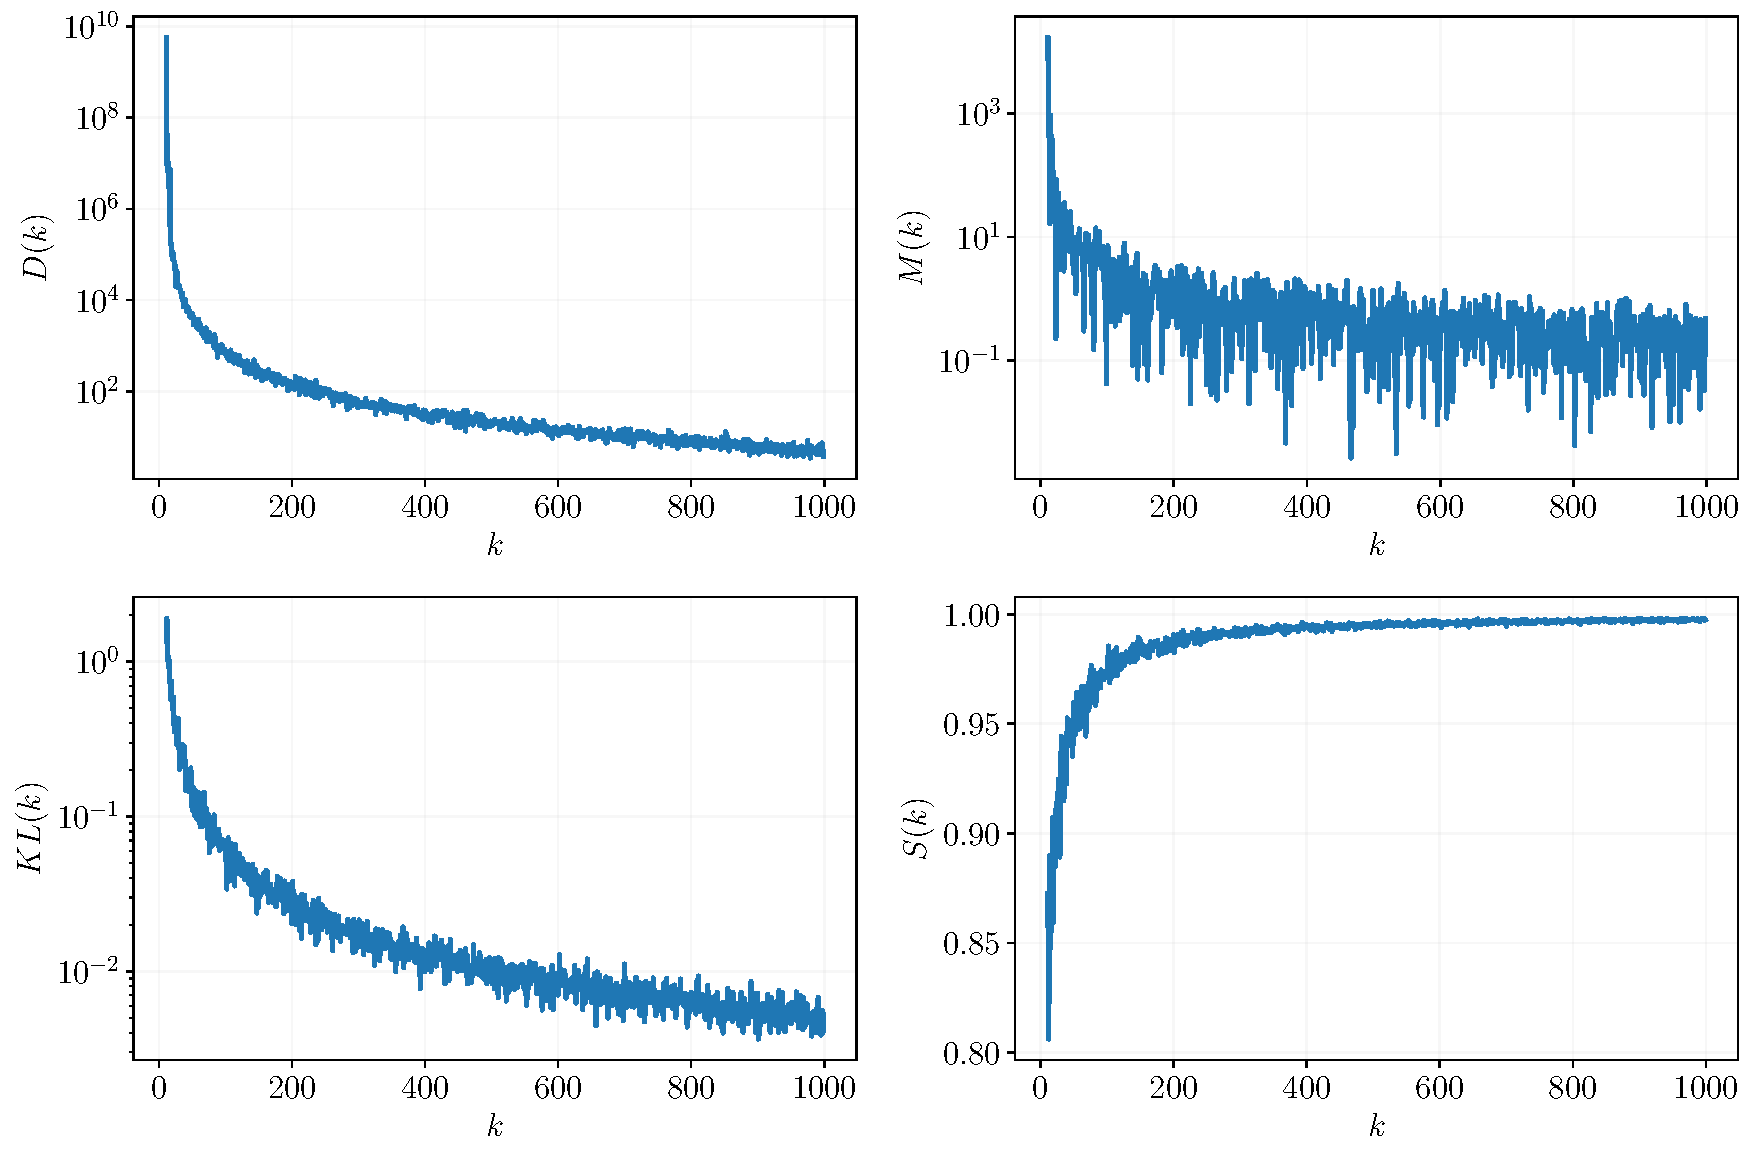
\includegraphics[width=0.75\textwidth]{paper/figures/synthetic-regression-functions.pdf}
    \end{figure}
    \vfill
    Функции стремятся к своим теоретическим пределам.
\end{frame}
%=======
\begin{frame}{Определение достаточного размера выборки}
    Синтетические данные сгенерированы из модели \underline{линейной} регрессии. Число объектов 1000, число признаков 20. Из данной выборки последовательно удаляется по одному объекту. Такой процесс повторяется $B=1000$ раз.
    \vfill
    \begin{figure}[h!]
        \centering
        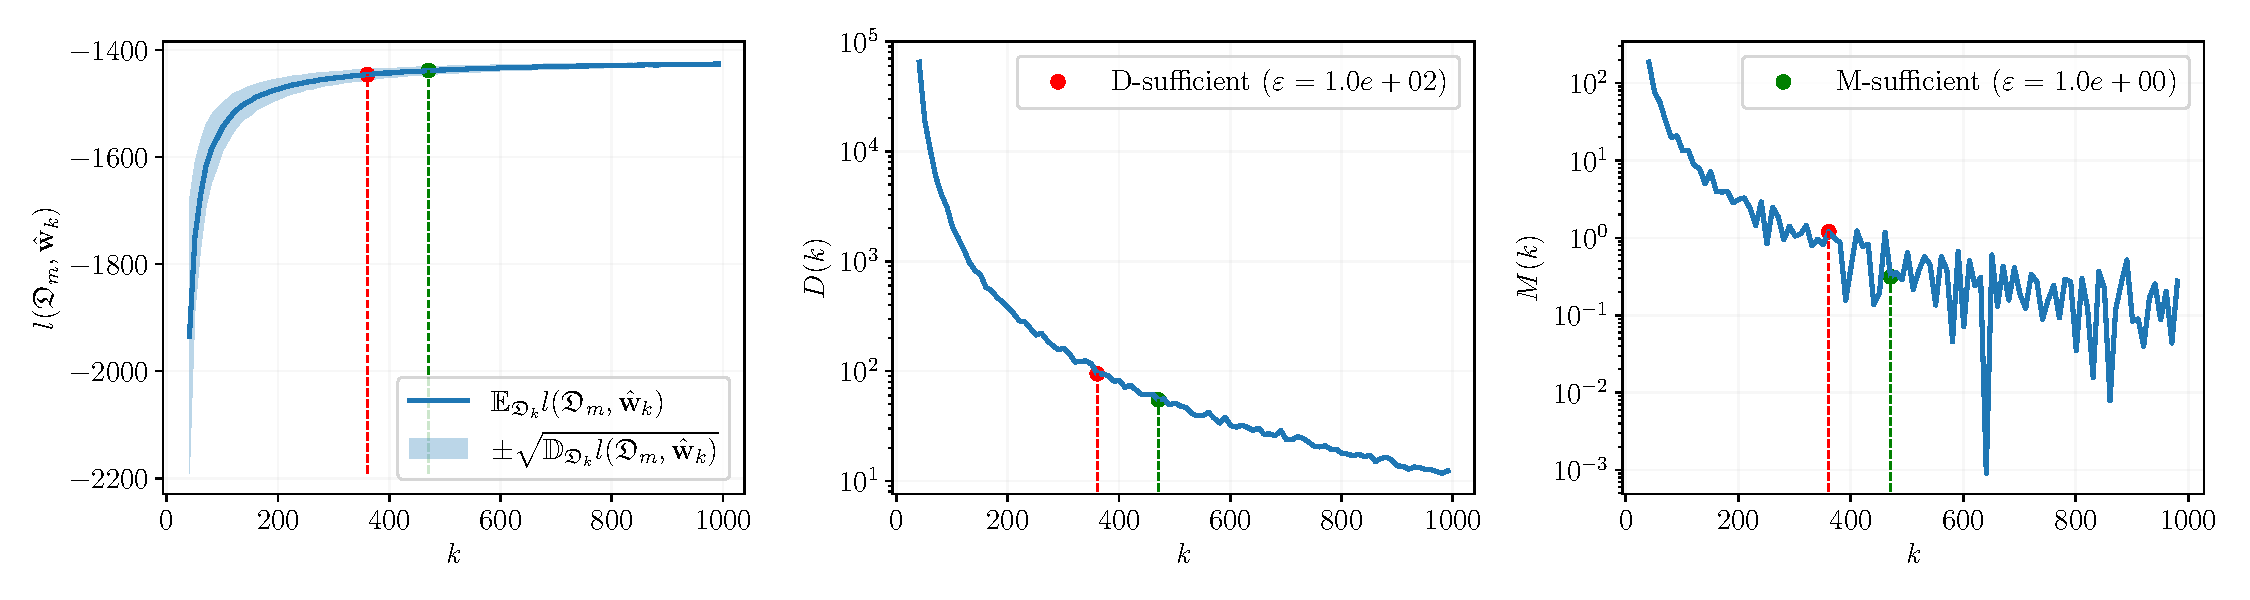
\includegraphics[width=\textwidth]{paper/figures/synthetic-regression-sufficient.pdf}
    \end{figure}
    \vfill
    На графиках указаны D-достаточный и M-достаточный размеры выборки. Для D-достаточности выбрано $\varepsilon = 3 \cdot 10^{1}$, для M-достаточности $\varepsilon = 4 \cdot 10^{-1}$.
\end{frame}
%=======
\begin{frame}{Определение достаточного размера выборки}
    Синтетические данные сгенерированы из модели \underline{логистической} регрессии. Число объектов 1000, число признаков 20. Из данной выборки последовательно удаляется по одному объекту. Такой процесс повторяется $B=1000$ раз.
    \vfill
    \begin{figure}[h!]
        \centering
        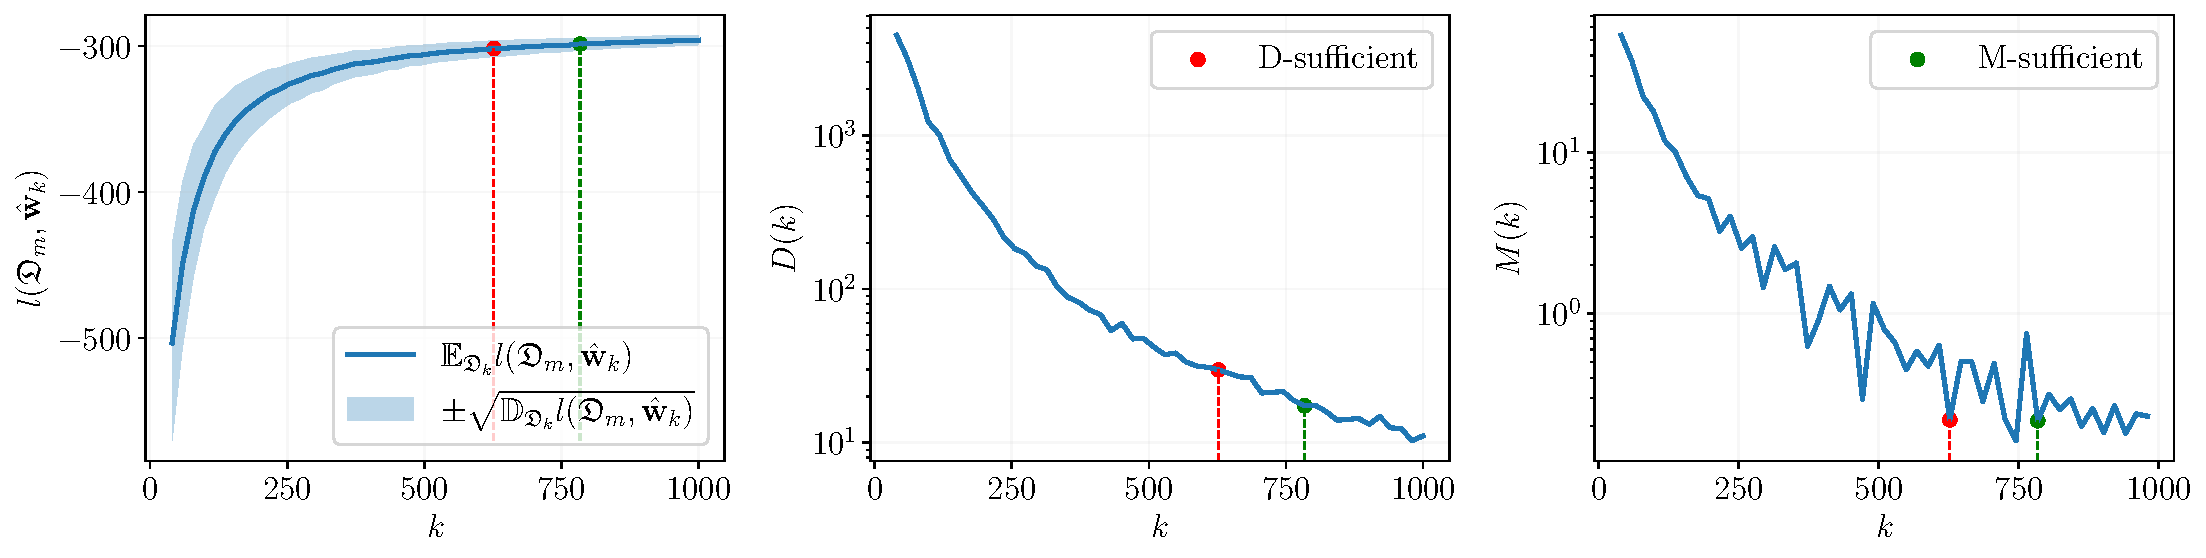
\includegraphics[width=\textwidth]{paper/figures/synthetic-classification-sufficient.pdf}
    \end{figure}
    \vfill
    На графиках указаны D-достаточный и M-достаточный размеры выборки. Для D-достаточности выбрано $\varepsilon = 3 \cdot 10^{1}$, для M-достаточности $\varepsilon = 6 \cdot 10^{-1}$.
\end{frame}
%=======
\begin{frame}{Определение достаточного размера выборки}
    Используется датасет Abalone с задачей регрессии из открытой библиотеки UCI\footnote{\href{https://archive.ics.uci.edu}{Markelle Kelly, Rachel Longjohn, Kolby Nottingham, The UCI Machine Learning Repository.}}. Число объектов 4177, число признаков 8. Из данной выборки последовательно удаляется по одному объекту. Такой процесс повторяется $B=1000$ раз.
    \vfill
    \begin{figure}[h!]
        \centering
        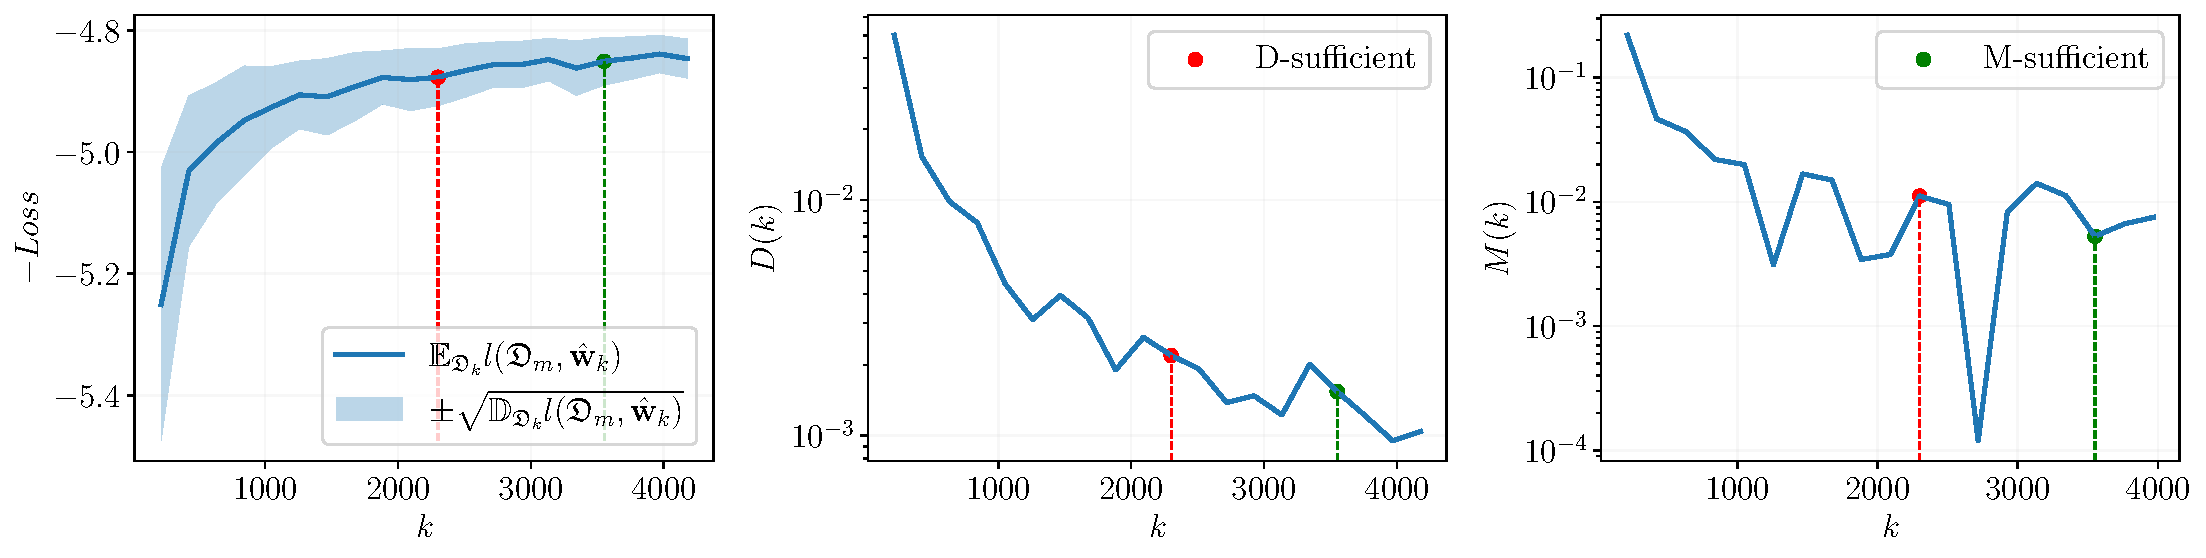
\includegraphics[width=\textwidth]{paper/figures/abalone-sufficient.pdf}
    \end{figure}
    \vfill
    На графиках указаны D-достаточный и M-достаточный размеры выборки. Для D-достаточности выбрано $\varepsilon = 2.5 \cdot 10^{-3}$, для M-достаточности $\varepsilon = 8 \cdot 10^{-3}$.
\end{frame}
%=======
\begin{frame}{Определение параметрического семейства функций с помощью генетического алгоритма}
    Анализируются датасеты с задачей \underline{регрессии} из открытой библиотеки UCI\footnote{\href{https://archive.ics.uci.edu}{Markelle Kelly, Rachel Longjohn, Kolby Nottingham, The UCI Machine Learning Repository.}}. Усреднение проводится по $B=100$ бутстрап-подвыборкам.
    \vfill
    \begin{figure}[h!]
        \centering
        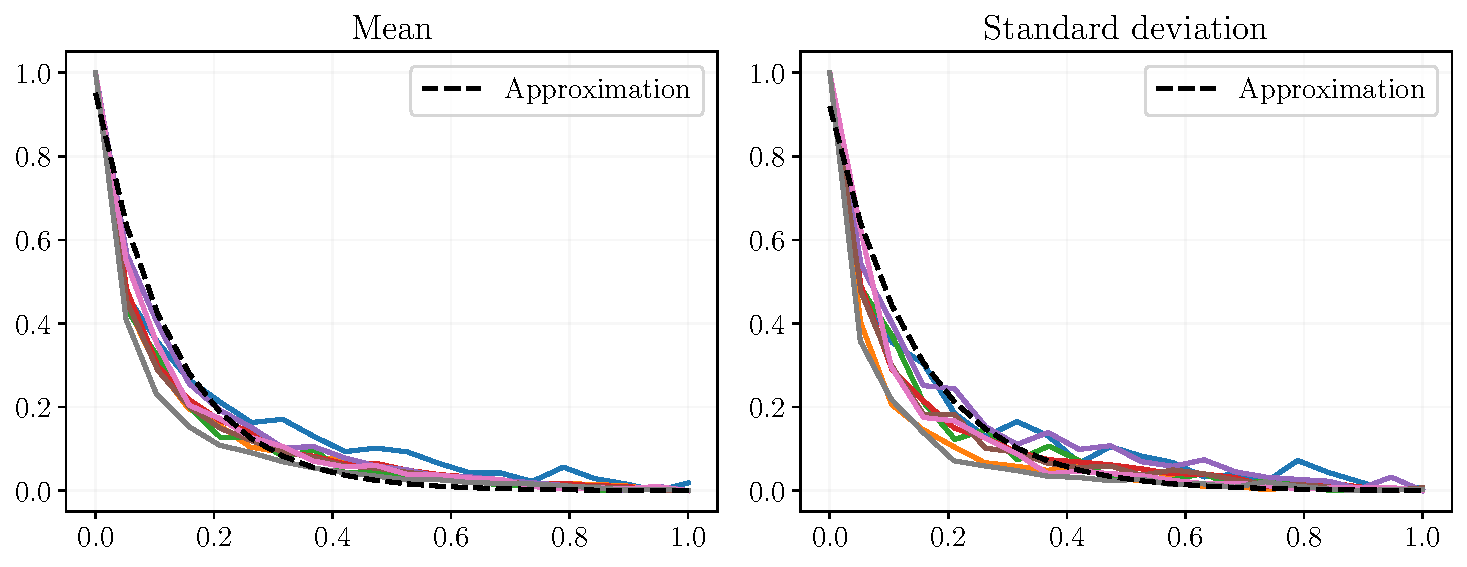
\includegraphics[width=\textwidth]{paper/figures/datasets_regression.pdf}
    \end{figure}
    \vfill
    Применение генетического алгоритма приводит к семейству функций
    \[ w_0 + w_1 \cdot \exp(w_2 \cdot x). \]
\end{frame}
%=======
\begin{frame}{Определение параметрического семейства функций с помощью генетического алгоритма}
    Анализируются датасеты с задачей \underline{классификации} из открытой библиотеки UCI\footnote{\href{https://archive.ics.uci.edu}{Markelle Kelly, Rachel Longjohn, Kolby Nottingham, The UCI Machine Learning Repository.}}. Усреднение проводится по $B=100$ бутстрап-подвыборкам.
    \vfill
    \begin{figure}[h!]
        \centering
        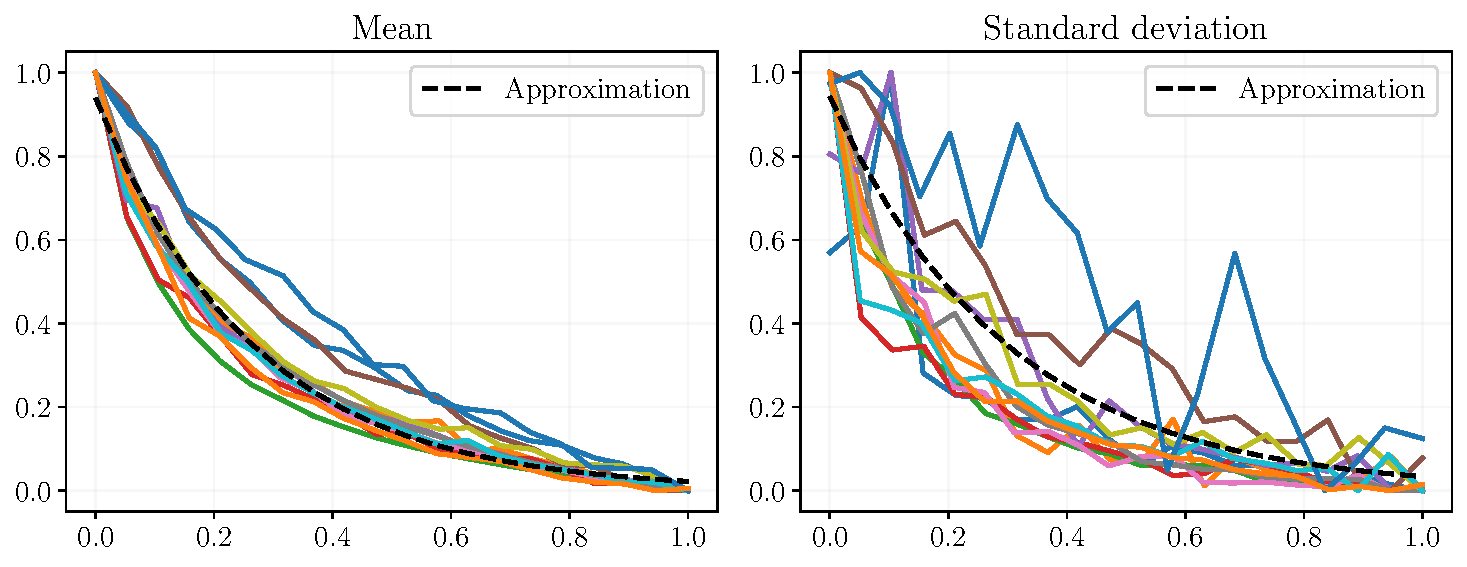
\includegraphics[width=\textwidth]{paper/figures/datasets_classification.pdf}
    \end{figure}
    \vfill
    Применение генетического алгоритма приводит к семейству функций
    \[ w_0 + w_1 \cdot \exp(w_2 \cdot x). \]
\end{frame}
%=======
\begin{frame}{Прогнозирование функции правдоподобия}
    Среднее значение и дисперсия аппроксимированы параметрическим семейством функций, полученным ранее. Производилось разделение на обучающую и тестовую выборки в соотношении 70:30. Аппроксимация производилась только на обучающей части. Достаточный размер выборки находился в тестовой части.
    \vfill
    \begin{block}{Синтетическая выборка (линейная регрессия)}
        \begin{figure}[h!]
            \centering
            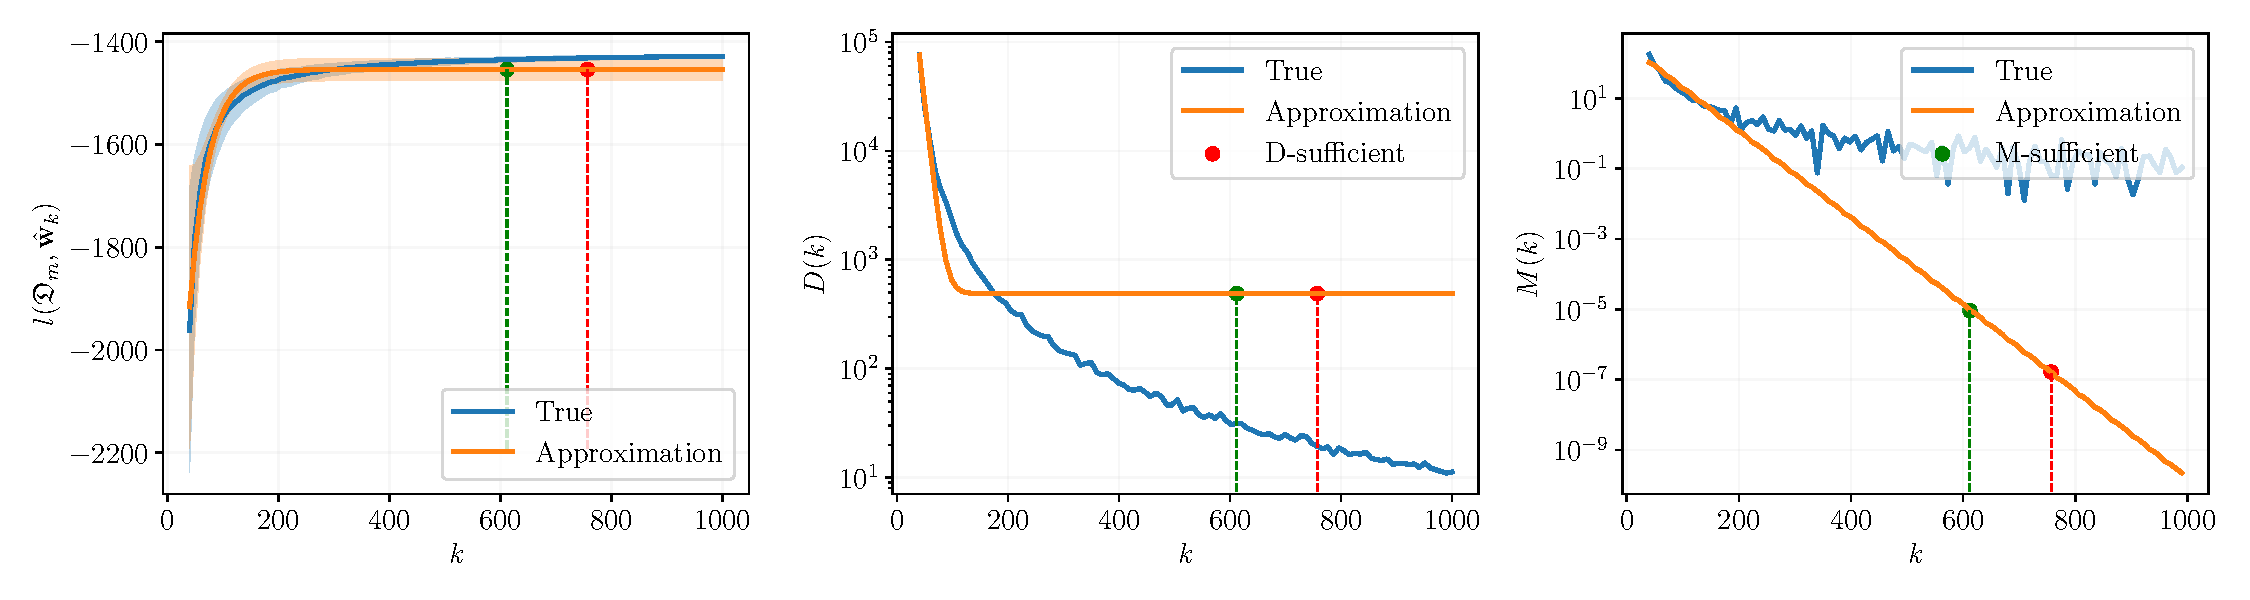
\includegraphics[width=\textwidth]{paper/figures/synthetic-regression-approximation.pdf}
        \end{figure}
    \end{block}
\end{frame}
%=======
\begin{frame}{Прогнозирование функции правдоподобия}
    \begin{block}{Синтетическая выборка (логистическая регрессия)}
        \begin{figure}[h!]
            \centering
            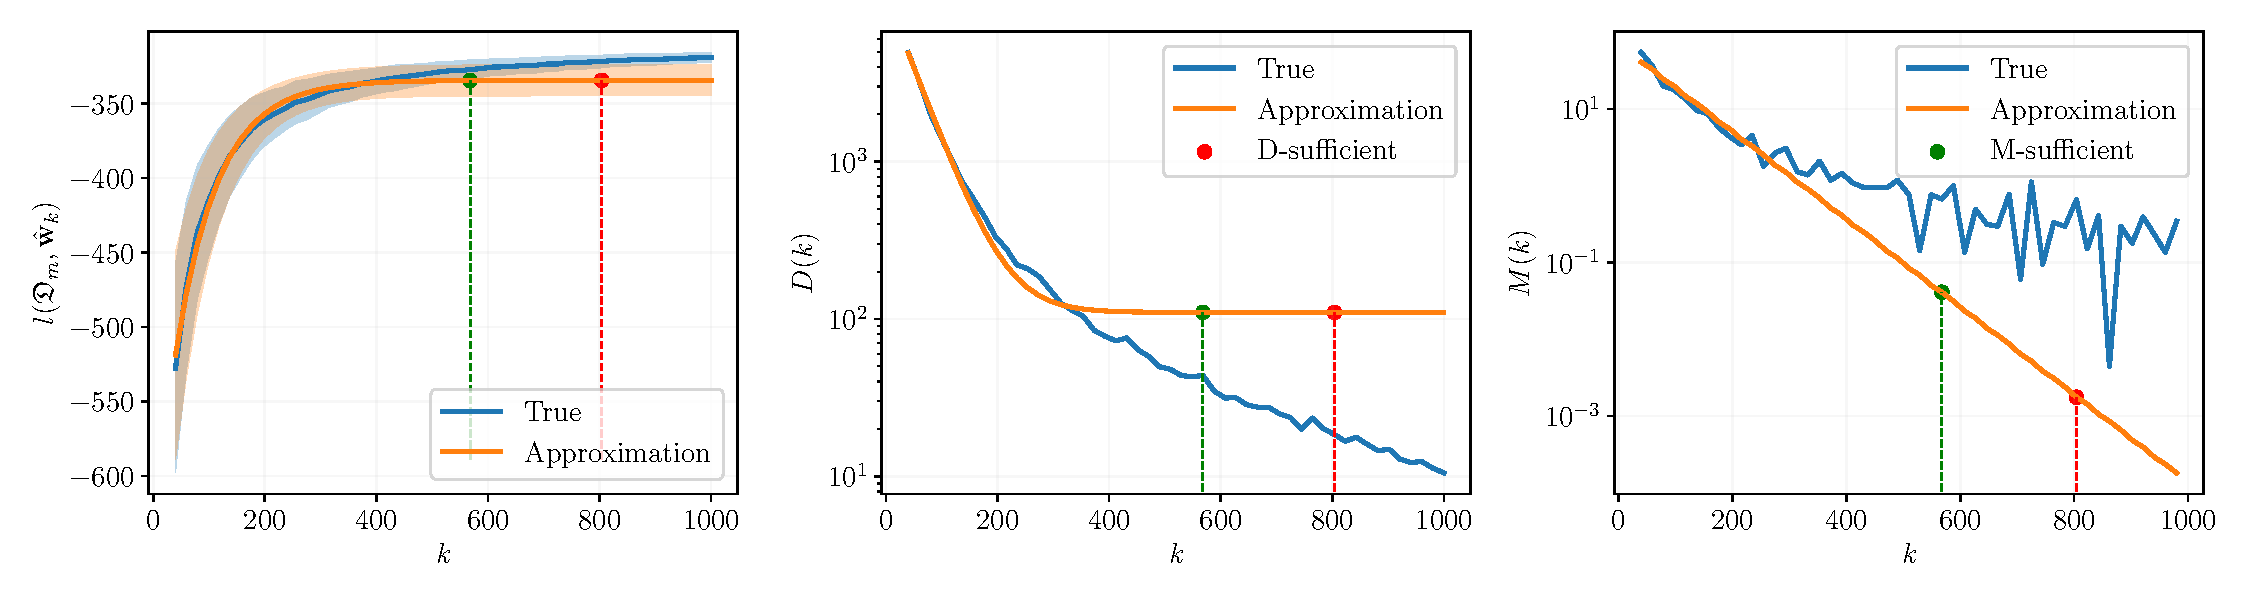
\includegraphics[width=\textwidth]{paper/figures/synthetic-classification-approximation.pdf}
        \end{figure}
    \end{block}
    \vfill
    \begin{block}{Выборка Abalone (регрессия)}
        \begin{figure}[h!]
            \centering
            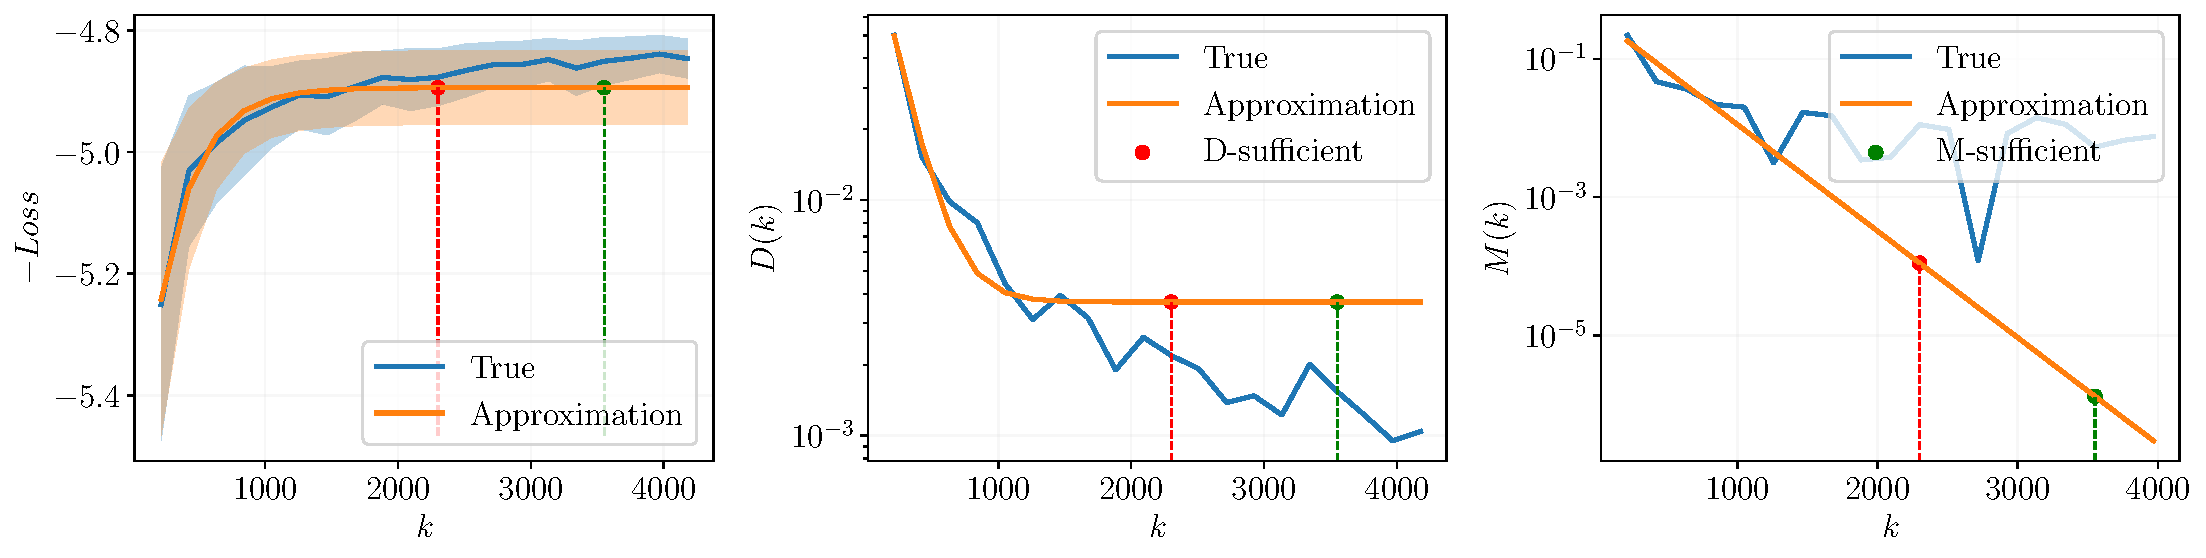
\includegraphics[width=\textwidth]{paper/figures/abalone-approximation.pdf}
        \end{figure}
    \end{block}
\end{frame}
%=======
\begin{frame}{Заключение}
    \begin{itemize}
        \item Предложены подходы к определению достаточного размера выборки на основе функции правдоподобия и апостериорных распределений.
        \item Доказана корректность подходов при определенных ограничениях на модель.
        \item Предложен метод прогнозирования функции правдоподобия при недостаточном размере выборки.
        \item Проведен вычислительный эксперимент для анализа методов.
        \item Определено параметрическое семейство функций, аппроксимирующее функцию ошибки для различных датасетов.
    \end{itemize}
\end{frame}
%=======
%\begin{frame}{Выносится на защиту}
%    \begin{enumerate}
%        \item Это первое...
%        \vfill
%        \item Это второе...
%        \vfill
%        \item Это третье...
%    \end{enumerate}
%\end{frame}
%=======

\end{document} 